\section{Consultar Tratamientos}

Un auxiliar tendrá una lista con todos los tratamientos de sus pacientes, tanto los que están en estado activo, incompleto, interrumpido y terminado. De esta manera sabrá cuantos y cuáles son sus tratamientos, su estado y la información de estos, como nombre de tratamiento, paciente al que se le expidió, fecha de expedición y número de medicamentos.

\subsubsection{Procedimiento}
\begin{enumerate}
	
	\item Da clic en el icono \textbf{Pacientes} de la pantalla \textbf{Menú Principal del Auxiliar}.

		\begin{figure}[!htbp]			\hypertarget{fig:mpAuxiliar3}{\hspace{1pt}}
		\begin{center}
			\includegraphics[height=0.4\textheight]{images/Iconos/Advertencia}
			\caption{Menú Principal del Auxiliar}
			\label{fig:mpAuxiliar3}
		\end{center}
	\end{figure}

	\item Se mostrará la pantalla \textbf{Pacientes}. 
	\newpage
	\begin{figure}[!htbp]			
		\hypertarget{fig:Auxiliares}{\hspace{1pt}}
		\begin{center}
			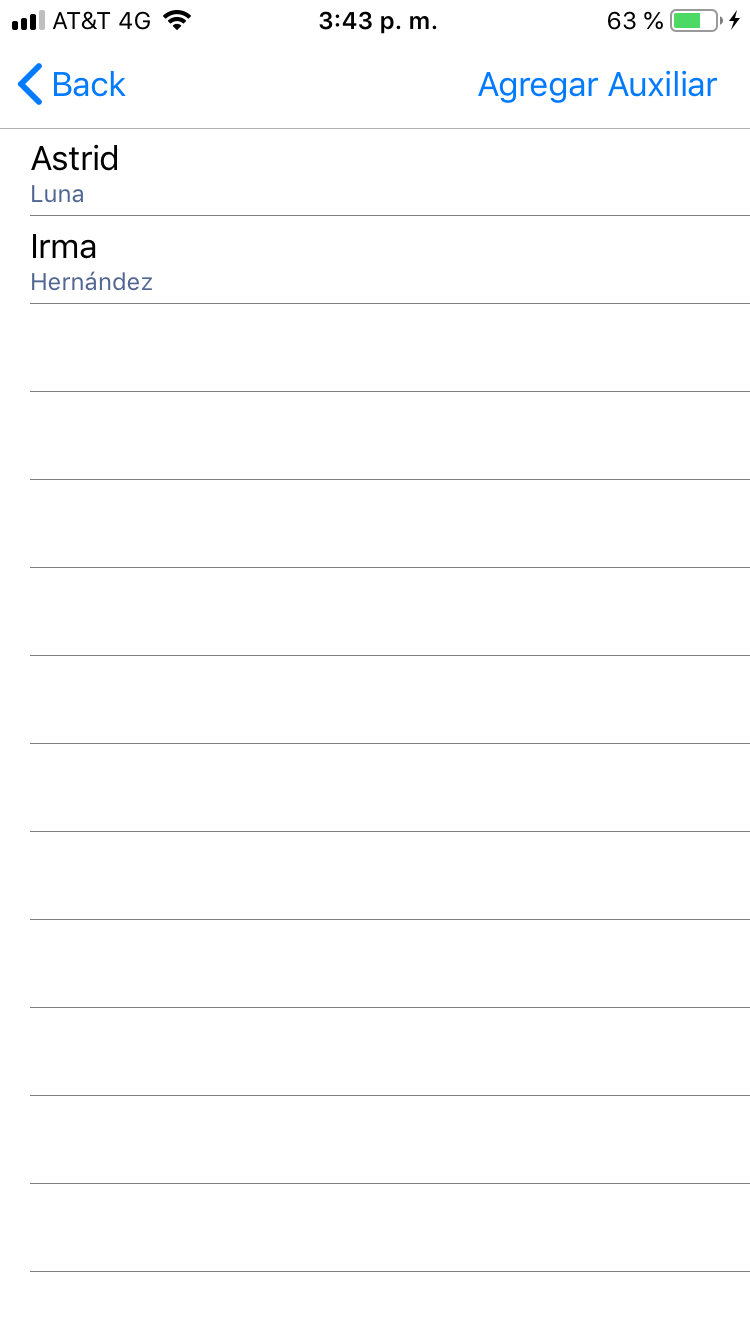
\includegraphics[height=0.4\textheight]{Paciente/AgregarAuxiliar/images/Auxiliares}
			\caption{Auxiliares}
			\label{fig:Auxiliares}
		\end{center}
	\end{figure}

	\item Selecciona el paciente de quien quieres consultar su tratamiento.


\end{enumerate}

